\documentclass[8pt, landscape, a4paper]{extarticle}

% --- 核心宏包 ---
\usepackage[UTF8]{ctex}
\usepackage[margin=0.8cm, top=1cm, bottom=1.3cm]{geometry}
\usepackage{multicol}
\usepackage{xcolor}
\usepackage{tcolorbox}
\usepackage{enumitem}
\usepackage{amsmath}
\usepackage{amssymb}
\usepackage{fontspec}
\usepackage{tikz}
\usetikzlibrary{arrows.meta, shapes}

% --- 去掉页码 ---
\pagestyle{empty}

% --- 颜色定义 (Blue 主题) ---
\definecolor{headerblue}{RGB}{41, 128, 185}    % Blue
\definecolor{navcolor}{RGB}{211, 84, 0}        % 导航橙
\definecolor{intuitioncolor}{RGB}{22, 160, 133}% 直觉绿
\definecolor{accentcolor}{RGB}{192, 57, 43}    % 强调红
\definecolor{section2}{RGB}{142, 68, 173}      % 紫色
\definecolor{dividergray}{RGB}{220, 220, 220}

% --- 全局设置 ---
\setlength{\parindent}{0pt}
\setlength{\columnsep}{0.4cm} 
\linespread{1.1} 

% --- 列表样式 ---
\setlist[itemize]{leftmargin=1.2em, nosep, itemsep=2pt, topsep=2pt, label=$\textcolor{headerblue}{\vcenter{\hbox{\tiny$\bullet$}}}$ }
\setlist[description]{leftmargin=0.2em, style=sameline, nosep, itemsep=2pt, font=\bfseries}

% --- Box 样式 ---
\newtcolorbox{mybox}[2][]{%
  colback=white,
  colframe=#2,
  coltitle=white,
  boxrule=1pt,             
  arc=2mm,                 
  left=4pt, right=4pt, top=3pt, bottom=3pt, 
  toptitle=3pt, bottomtitle=3pt, 
  fonttitle=\bfseries\sffamily\large,
  title={#1},
  after skip=5pt          
}

% --- 自定义命令 ---
\newcommand{\subt}[1]{{\vspace{2pt}\textbf{\large \textcolor{black}{#1}}}}

\newcommand{\boxdesc}[1]{%
    \textit{\small \textcolor{gray}{#1}}%
    \par\vspace{2pt}%
    {\color{dividergray}\hrule height 0.5pt}%
    \vspace{2pt}%
}

\newcommand{\sepline}{%
    \par \vspace{3pt}%
    {\color{dividergray}\hrule height 0.5pt}%
    \par \vspace{3pt}%
}

% 公式间距
\setlength{\abovedisplayskip}{3pt}
\setlength{\belowdisplayskip}{3pt}

\begin{document}

% --- 页眉 ---
\begin{center}
    {\Huge \textbf{\sffamily \textcolor{headerblue}{傅里叶变换 Fourier Transforms Cheat Sheet}}} \\
    \vspace{0.2cm}
    {\large \texttt{The Prism of Mathematics: Decomposing the Universe into Waves}}
\end{center}

% --- 开始四栏布局 ---
\begin{multicols*}{4}

% === 第一栏 ===

\begin{mybox}[️ 场景导航 (Use Cases)]{navcolor}
    \boxdesc{遇到什么问题 $\to$ 用什么工具}
    \begin{itemize}[itemsep=2pt]
        \item \textbf{音频降噪/均衡} $\to$ 频域滤波 (Low/High Pass)
        \item \textbf{图像压缩 (JPEG)} $\to$ DCT (离散余弦变换)
        \item \textbf{大整数乘法} $\to$ 卷积定理 + FFT
        \item \textbf{解微分方程} $\to$ 频域代数化
        \item \textbf{量子力学} $\to$ 位置/动量对偶 (海森堡)
        \item \textbf{CT 扫描} $\to$ Radon 变换 (傅里叶切片)
    \end{itemize}
\end{mybox}

\begin{mybox}[1. 连续傅里叶 (CTFT)]{headerblue}
    \boxdesc{时域与频域的桥梁}
    
    \subt{正变换 (Analysis)}
    $$ F(\omega) = \int_{-\infty}^{\infty} f(t) e^{-i\omega t} dt $$
    \textit{含义: 信号 $f(t)$ 中包含多少频率为 $\omega$ 的成分。}
    \sepline
    
    \subt{逆变换 (Synthesis)}
    $$ f(t) = \frac{1}{2\pi} \int_{-\infty}^{\infty} F(\omega) e^{i\omega t} d\omega $$
    \textit{含义: 所有频率成分叠加还原回信号。}
    \sepline
    
    \subt{狄拉克 $\delta$ 函数}
    \begin{itemize}
        \item $\delta(t) \iff 1$ (脉冲包含所有频率)
        \item $1 \iff 2\pi \delta(\omega)$ (直流是 0 频率)
        \item $e^{i\omega_0 t} \iff 2\pi \delta(\omega - \omega_0)$
    \end{itemize}
\end{mybox}

\begin{mybox}[2. 核心性质 (Properties)]{headerblue}
    \boxdesc{在频域操作更简单}
    
    \subt{卷积定理 (Convolution)}
    \textbf{时域卷积 = 频域相乘}
    $$ f(t) * g(t) \iff F(\omega) \cdot G(\omega) $$
    \textit{威力: $O(N^2)$ 的卷积变为 $O(N \log N)$ 的乘法。}
    \sepline
    
    \subt{微分性质}
    $$ f'(t) \iff i\omega F(\omega) $$
    \textit{威力: 微分方程变为代数方程。}
    \sepline
    
    \subt{帕塞瓦尔定理 (Parseval)}
    能量守恒:时域总能量 = 频域总能量。
    $$ \int |f(t)|^2 dt = \frac{1}{2\pi} \int |F(\omega)|^2 d\omega $$
\end{mybox}

\columnbreak

% === 第二栏 ===

\begin{mybox}[3. 离散傅里叶 (DFT)]{headerblue}
    \boxdesc{计算机里的傅里叶}
    
    \subt{定义}
    对于长度为 $N$ 的序列 $x[n]$:
    $$ X[k] = \sum_{n=0}^{N-1} x[n] e^{-i\frac{2\pi}{N}kn} $$
    \begin{itemize}
        \item $k$: 频率索引 ($0 \dots N-1$)。
        \item $e^{-i\frac{2\pi}{N}}$: $N$ 次单位根 $W_N$。
    \end{itemize}
    \sepline
    
    \subt{采样定理 (Nyquist)}
    采样频率必须大于信号最高频率的 2 倍 ($f_s > 2f_{max}$),否则会发生\textbf{混叠 (Aliasing)}。
    \sepline
    
    \subt{频谱泄露 (Leakage)}
    如果信号周期不是 $N$ 的整数倍,能量会泄露到相邻频率。
    \textit{解法: 加窗 (Windowing),如 Hamming 窗。}
\end{mybox}

\begin{mybox}[4. 快速傅里叶变换 (FFT)]{headerblue}
    \boxdesc{20世纪最重要的算法}
    
    \subt{Cooley-Tukey 算法}
    利用 $W_N^k$ 的对称性和周期性,分治求解。
    $$ DFT(N) \to 2 \times DFT(N/2) + O(N) $$
    \begin{itemize}
        \item \textbf{复杂度}: $O(N^2) \to O(N \log N)$。
        \item \textbf{蝶形运算}: 基本计算单元。
    \end{itemize}
    \sepline
    
    \subt{应用: 多项式乘法}
    两个 $N$ 次多项式相乘。
    \begin{enumerate}
        \item 系数转点值 (FFT)。
        \item 点值相乘 ($O(N)$)。
        \item 点值转系数 (IFFT)。
    \end{enumerate}
\end{mybox}

\columnbreak

% === 第三栏 ===

\begin{mybox}[5. 相关变换 (Relatives)]{headerblue}
    \boxdesc{傅里叶家族}
    
    \subt{短时傅里叶 (STFT)}
    加窗,看\textbf{局部}频率随时间的变化 (声纹图)。
    $$ X(m, \omega) = \sum x[n] w[n-m] e^{-i\omega n} $$
    \textit{缺陷: 窗口大小固定,时频分辨率不可兼得 (测不准)。}
    \sepline
    
    \subt{小波变换 (Wavelet)}
    用不同尺度的波 (小波) 去拟合。
    \textit{优势: 高频处时间分辨率高,低频处频率分辨率高。}
    \sepline
    
    \subt{离散余弦变换 (DCT)}
    只用实数余弦 (丢掉虚部)。
    \textit{应用: JPEG 压缩 (能量集中在低频)。}
\end{mybox}

\begin{mybox}[6. 物理直觉 (Physics)]{headerblue}
    \boxdesc{自然界的语言}
    
    \subt{不确定性原理}
    $$ \Delta t \cdot \Delta \omega \ge \frac{1}{2} $$
    信号在时域越窄 (短),在频域就越宽 (广)。
    \textit{量子力学: $\Delta x \Delta p \ge \hbar/2$ 本质上就是傅里叶变换性质。}
    \sepline
    
    \subt{衍射与成像}
    透镜的焦平面就是物体的傅里叶变换平面。
    晶体衍射图样就是晶格的倒易空间 (频域)。
\end{mybox}

\begin{mybox}[7. Python / Numpy 实战]{headerblue}
    \boxdesc{代码工具箱}
    \begin{itemize}
        \item \texttt{np.fft.fft(x)}: 计算 FFT。
        \item \texttt{np.fft.fftfreq(n, d)}: 获取频率轴坐标。
        \item \texttt{np.fft.fftshift(X)}: 将零频移到中心。
        \item \textbf{滤波}: \texttt{X[high\_freqs] = 0; ifft(X)}。
    \end{itemize}
\end{mybox}

\columnbreak

% === 第四栏 ===

\begin{mybox}[8. 高阶技巧 (Advanced)]{headerblue}
    \boxdesc{魔改与优化}
    
    \subt{分数阶傅里叶 (FRFT)}
    旋转时频平面 $\alpha$ 角度。
    \textit{应用: 线性调频信号 (Chirp) 处理。}
    \sepline
    
    \subt{数论变换 (NTT)}
    在有限域 $GF(p)$ 上做 FFT。
    \textit{优势: 无浮点误差。应用: 大数乘法库 (GMP), 密码学 (Lattice)。}
    \sepline
    
    \subt{压缩感知 (Compressed Sensing)}
    如果信号在频域稀疏,可以低于奈奎斯特频率采样并恢复。
    $$ \min \|x\|_1 \quad \text{s.t.} \quad y = \Phi x $$
\end{mybox}

\vspace*{\fill}

\begin{mybox}[ 核心直觉 (Intuition)]{intuitioncolor}
    \boxdesc{“万物皆震荡。”}
    
    % TikZ 矢量图: 时域方波 -> 频域 Sinc 函数
    \begin{center}
    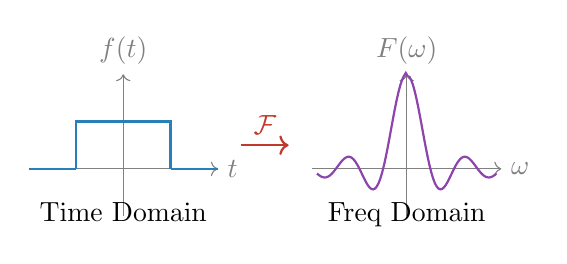
\begin{tikzpicture}[scale=0.6]
        % 时域
        \begin{scope}[xshift=-3cm]
            \draw[->, gray] (-2,0) -- (2,0) node[right] {$t$};
            \draw[->, gray] (0,-1) -- (0,2) node[above] {$f(t)$};
            \draw[thick, headerblue] (-1,0) -- (-1,1) -- (1,1) -- (1,0);
            \draw[thick, headerblue] (-2,0) -- (-1,0);
            \draw[thick, headerblue] (1,0) -- (2,0);
            \node[below] at (0,-0.5) {Time Domain};
        \end{scope}
        
        % 箭头
        \draw[->, thick, accentcolor] (-0.5, 0.5) -- (0.5, 0.5) node[midway, above] {$\mathcal{F}$};
        
        % 频域
        \begin{scope}[xshift=3cm]
            \draw[->, gray] (-2,0) -- (2,0) node[right] {$\omega$};
            \draw[->, gray] (0,-1) -- (0,2) node[above] {$F(\omega)$};
            \draw[thick, section2, domain=-1.9:1.9, samples=100] plot (\x, {sin(180*\x*2)/(3.14*\x+0.001)});
            \node[below] at (0,-0.5) {Freq Domain};
        \end{scope}
    \end{tikzpicture}
    \end{center}

    \hspace{1em}傅里叶变换不仅仅是一个数学公式,它是一种\textbf{世界观}。
    \vspace{4pt}
    
    \subt{三大核心视角}
    \begin{itemize}[itemsep=4pt]
        \item \textbf{正交分解}: 
        正弦波 $e^{i\omega t}$ 是函数空间的一组正交基。傅里叶变换就是把信号投影到这组基上,求坐标 (系数)。
        
        \item \textbf{全局性}: 
        频域上的一个点,对应时域上的无限长正弦波。修改频域的一点,会影响时域的所有时刻。
        
        \item \textbf{对偶性}: 
        时域的卷积等于频域的乘法。时域的离散对应频域的周期。时域的压缩对应频域的扩展。两个世界完美对称。
    \end{itemize}
    
    \vspace{6pt}
    \centering\textit{\footnotesize 给我足够多的正弦波,我可以构造出整个宇宙。}
\end{mybox}

\end{multicols*}

\end{document}
